\chapter{Implementação e Testes do Aplicativo} \label{cap:development}
Neste capítulo, são apresentados os detalhes de implementação e testes do aplicativo. 

% **********************
% Integração de Sistemas
% **********************
\section{Integração de Sistemas}
O desenvolvimento da aplicação evolveu a integração de múltiplos sistemas de software, tanto internos quanto externos. Nesta secção, primeiro é apresentada a integração com o sistema de back-end, desenvolvido internamente. Em seguida, o mesmo é feito para os sistemas externos. Por último, a ferramenta utilizada para testes das integrações feitas por RESTful API's são apresentadas. 

\subsection{Back-end}
A integração com o back-end foi feita por meio de uma API REST. A API fornece endpoints que retornam informações relacionadas à lógica de negócio da aplicação e permitem o cadastro de dados do usuário.

O formato utilizado para troca de dados foi o JSON \todo{referenciar fig json}. Este formato foi utilizado por apresentar uma notação simples para entendimento e pelo fato de ser utilizado em larga escala em integrações de serviço web. Do ponto de vista humano, a notação é de fácil visualização por não apresentar uma sintaxe verbosa. Além disso, o formato tem suporte nativo de diversas linguagens de programação, incluindo o Swift, utilizado para realizar a implementação.

\missingfigure{exemplo de json}

A API contém algumas características relacionadas à segurança do sistema. A API fornece diferentes níveis de acesso para as chamadas a fim de proteger dados sensíveis. Todo usuário recebe um \textit{token} no momento em que realiza o login ou é registrado no aplicativo. Este \textit{token} é utilizado para realizar a autenticação de chamadas da API, permitindo a identificação do usuário que realizou a requisição pelo aplicativo. Através da identificação, o back-end pode retornar ou negar o pedido de chamada de API de acordo com o nível de acesso do usuário. Além da autenticação e autorização de usuários no sistema, existem dois ambientes de uso da API: um para fase de desenvolvimento e testes, outro para o aplicativo em produção. Ambos os ambientes contêm o mesmo conjunto de chamadas de API disponíveis, distinguindo-se apenas no uso de diferentes bancos de dados (desenvolvimento e produção). Este recurso permite a separação do uso do aplicativo para fins de testes, realizados pelo time de desenvolvimento e pelo cliente, e para fins de uso real, feito pelo usuário final. A separação dos ambientes é feita a partir da diferenciação da URL base da API REST.

No código do aplicativo, as chamadas de API são feitas com o auxílio de uma biblioteca para a linguagem Swift. A biblioteca, denominada Alamofire \todo{ref alamofire}, é uma camada de abstração para a utilização de recursos de rede do sistema iOS.

O recebimento dos dados da API é feita a partir de uma tradução automática do formato JSON para objetos do Swift. Através do recurso denominado \textit{Codable} da linguagem e da configuração de parâmetros de transformação de dados. Primeiramente, são escolhidos os agentes de codificação e decodificação para atender o formato JSON. Em seguida é utilizado o parâmetro de configuração que transforma a notação \textit{snake case} da API para a notação \textit{camel case}, utilizada no código \todo{ref fig snake camel}.

\subsection{Serviços Externos}
O desenvolvimento do aplicativo teve como requisito a implementação dos sistemas de geolocalização, pagamento e envio de SMS. No projeto, optou-se pela utilização destes sistemas na forma de serviços devido ao grande esforço envolvido na implementação e manutenção dos mesmos. Existem diversas alternativas consolidadas há anos no mercado para cada um dos sistemas citados. As soluções escolhidas e as integrações realizadas são apresentadas a seguir. 

\subsubsection{Geolocalização}
O aplicativo apresentou como um de seus requisitos funcionais a presença de um sistema de mapa, assim como a utilização da localização do usuário. Foi escolhido o serviço de geolocalização do Google Maps \todo{referenciar google maps api}, pelo motivo do mesmo disponibilizar uma SDK para o sistema iOS de fácil utilização, com boa documentação e suporte em comunidades da internet. Para detectar a localização do usuário, utilizou-se o recurso de GPS nativo do sistema iOS, disponibilizado através do framework \textit{Core Location}, parte da camada de \textit{Core Services} do sistema operacional.

O serviço de geolocalização do Google Maps é utilizado em diversas partes do aplicativo. No momento do cadastro de uma academia, o serviço é utilizado para o preenchimento do campo endereço (Figura \ref{fig:address-field}), obrigatório para todos os estabelecimentos cadastrados na plataforma. Requisições são feitas para a API do Google Maps à medida que o usuário acrescenta caracteres no campo de endereço. Como retorno, opções de endereços semelhantes ao digitado são apresentadas na interface (Figura \ref{fig:search-delfino}). Uma vez que o usuário escolhe um dos endereços disponíveis na busca, o serviço de geolocalização retorna as coordenadas referentes ao endereço. Estas coordenadas são enviadas ao back-end para armazenamento no banco de dados, junto aos demais dados da academia, e posteriormente são utilizadas para demarcação dos estabelecimentos no mapa.

\begin{figure}[H]
	\centering
    \begin{subfigure}[b]{0.4\textwidth}
        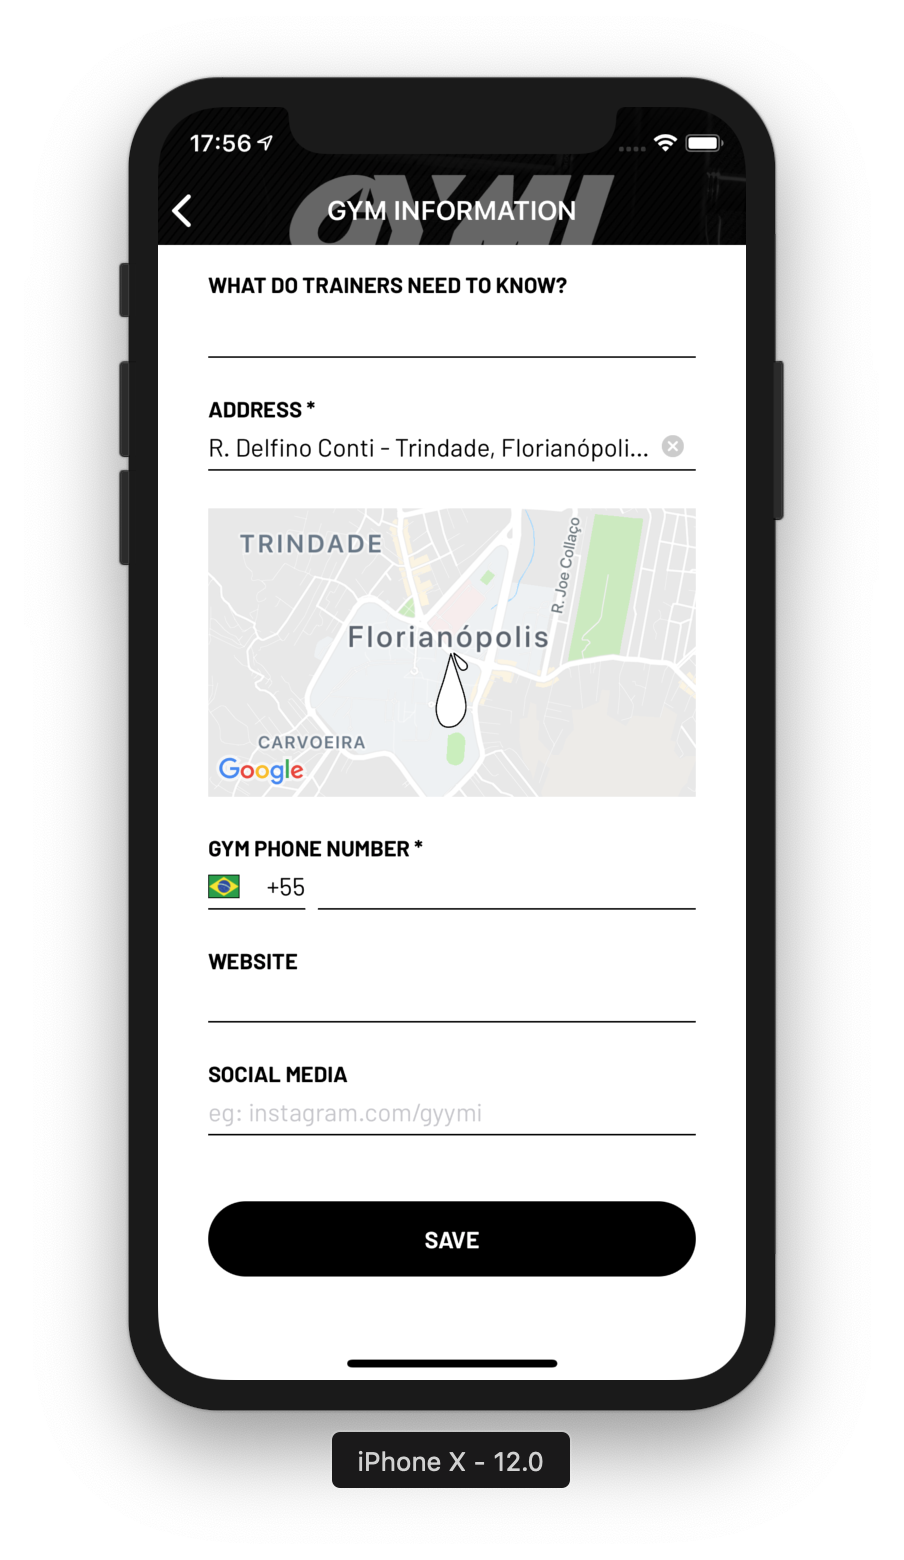
\includegraphics[width=\textwidth]{pfc/figuras/delfino-conti-2.png}
        \caption{Preenchimento do campo de endereço}
        \label{fig:address-field}
    \end{subfigure}
    ~
	\begin{subfigure}[b]{0.4\textwidth}
        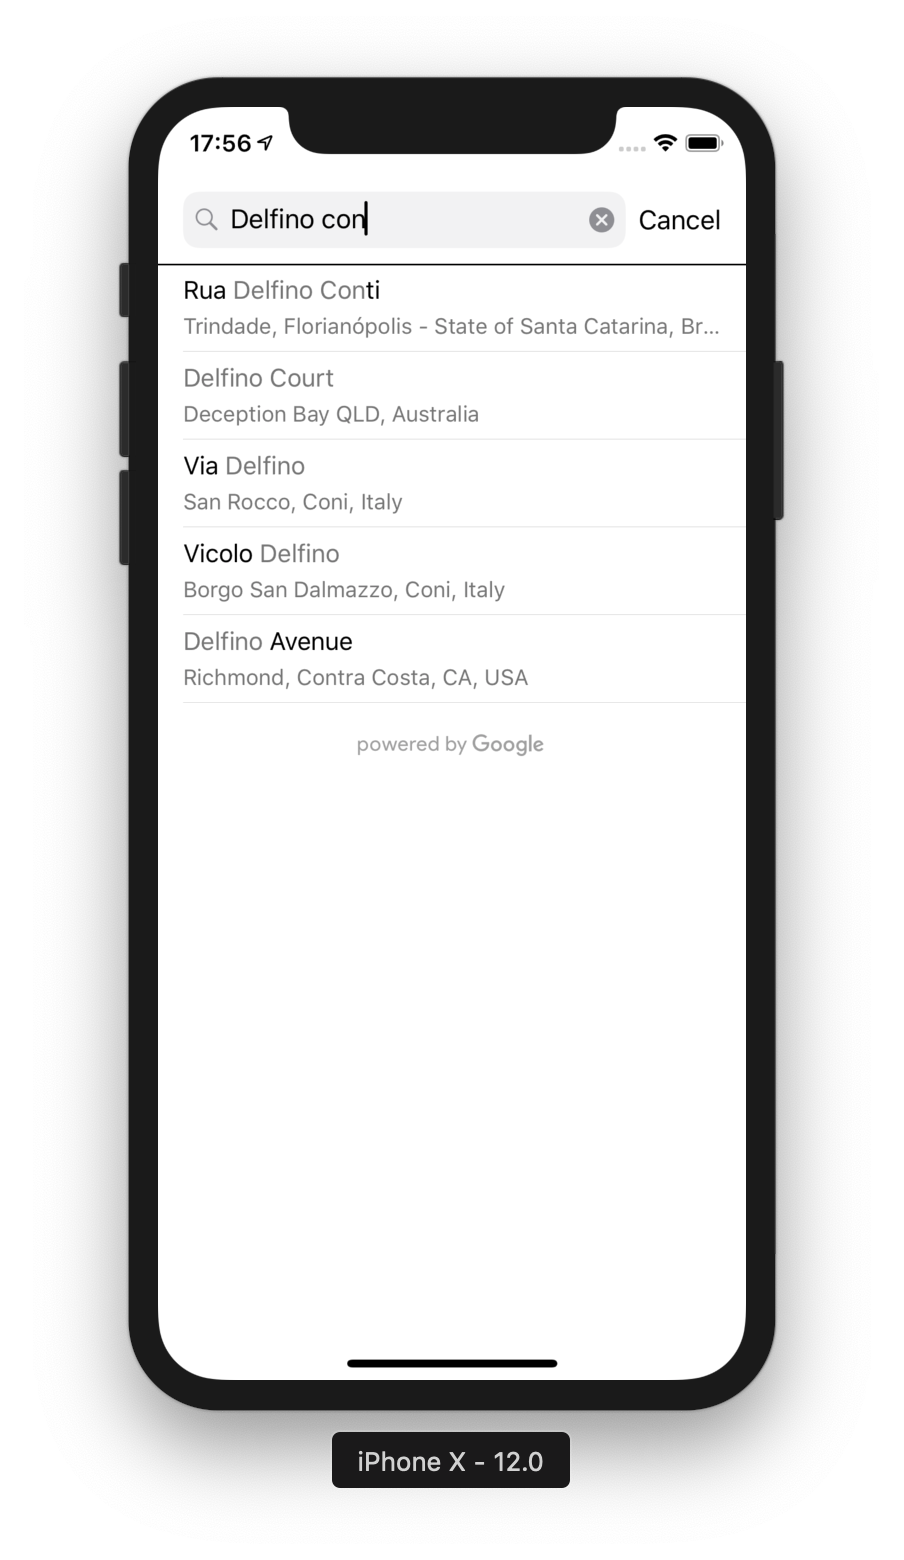
\includegraphics[width=\textwidth]{pfc/figuras/delfino-conti.png}
        \caption{Busca por endereços através da API do Google Maps}
        \label{fig:search-delfino}
    \end{subfigure}
    ~
    \caption{Etapa de preenchimento do campo endereço no cadastro de uma academia}
    \label{fig:addreess-field-fill}
\end{figure}

Outra utilização do serviço de geolocalização é o sistema de mapas, recorrente em diversas telas do aplicativo. O sistema de mapas é utilizado de maneira estática (sem a interação do usuário) nas telas de boas vindas (Figura \ref{fig:gym-welcome}), de perfil (Figuras \ref{fig:gym-profile} e \ref{fig:tr-gym-profile-view}) e de cadastro (Figura \ref{fig:address-field}) das academias e, também, na tela de confirmação de agendamento de treino (Figura \ref{fig:tr-booking-confirmed}). Na interface do treinador (Figura \ref{fig:tr-gym-search}), o mapa é renderizado na tela dinamicamente conforme a interação do usuário. O sistema de mapas permite a utilização de movimentos de pinça para alterar o zoom, além da movimentação simples do mapa através de toques na tela. Sempre que um mapa é renderizado na tela do aplicativo, uma requisição é feita ao back-end a fim de identificar as academias que estão presentes naquela região do mapa. O ponto central da região do mapa é enviado junto com um raio de busca (foi utilizado como padrão um raio de busca de $5\,km$) para o back-end. Então, uma lista com todas as academias da região é retornada e, a partir dos dados de coordenadas salvos, marcações são feitas no mapa.
                               
O framework \textit{Core Location} é utilizado em conjunto com o sistema de mapas para detectar a posição atual do usuário. Para utilizar o recurso nativo do sistema iOS, uma requisição de permissão de uso do sistema de localização do dispositivo deve ser feita ao usuário (Figura \ref{fig:gps-permission}). Em seguida, uma marcação especial é feita no mapa (ícone de músculos do braço - Figura \ref{fig:muscle-marker}) para indicar a localização corrente. A partir deste instante, um observador é configurado para que o sistema operacional emita um aviso ao aplicativo quando o usuário se movimentar. A configuração é feita com um parâmetro de precisão de $10/,m$. Assim, quando o usuário se desloca mais que esta distância, um aviso é emitido ao aplicativo e, em seguida, a posição do marcador no mapa é atualizada.

\begin{figure}[H]
	\centering
    \begin{subfigure}[b]{0.38\textwidth}
        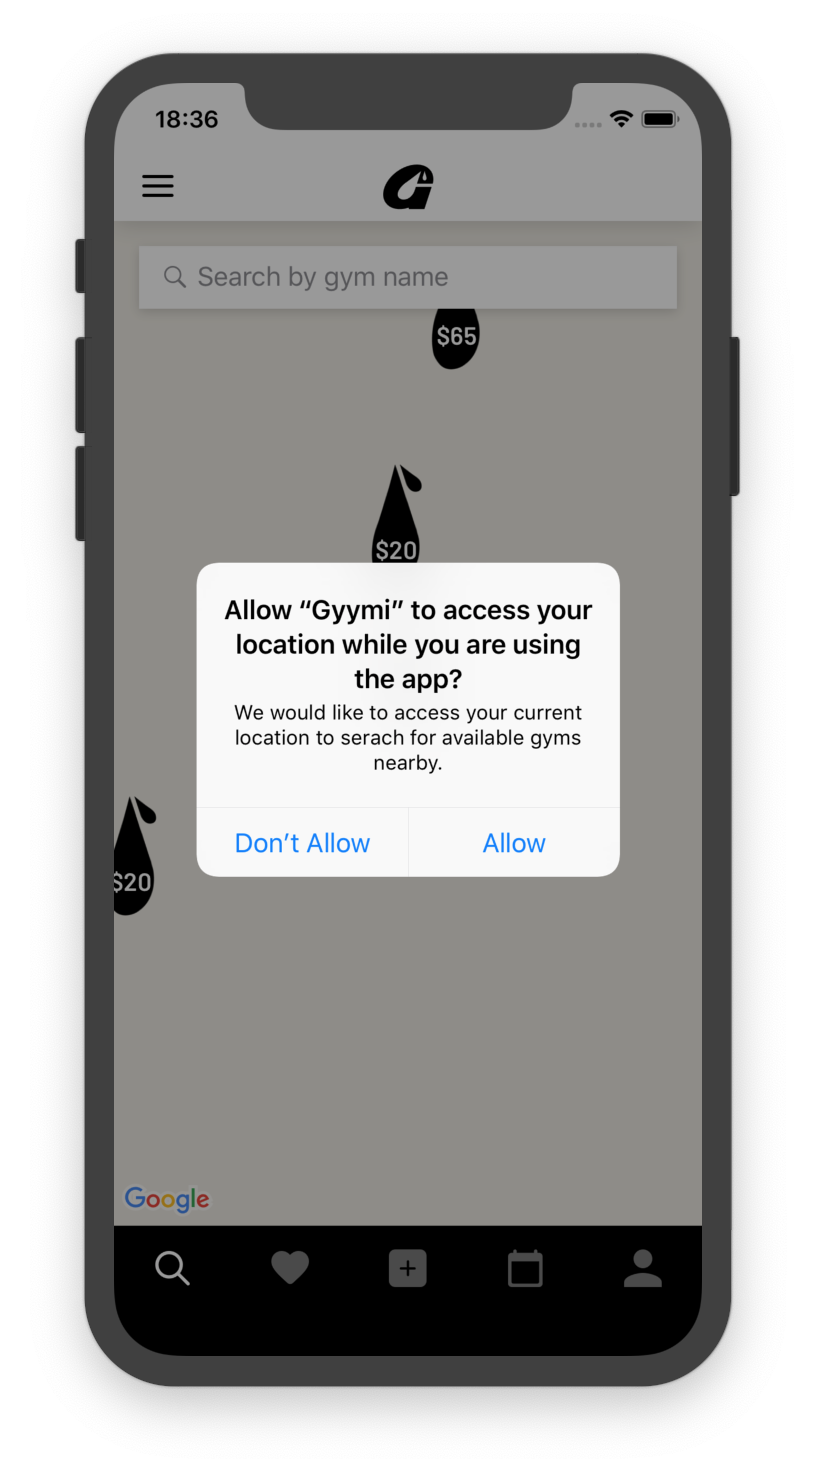
\includegraphics[width=\textwidth]{pfc/figuras/gps-permission.png}
        \caption{Permissão de uso do GPS}
        \label{fig:gps-permission}
    \end{subfigure}
    ~
	\begin{subfigure}[b]{0.4\textwidth}
        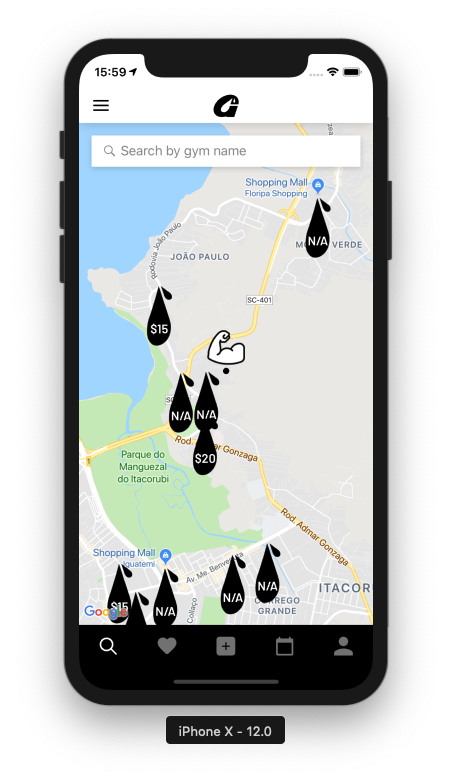
\includegraphics[width=\textwidth]{pfc/figuras/tr-home.png}
        \caption{Marcador de posição}
        \label{fig:muscle-marker}
    \end{subfigure}
    ~
    \caption{Marcação da posição atual do usuário no mapa}
    \label{fig:user-position}
\end{figure}

\subsubsection{Pagamento}
Um sistema de pagamentos foi utilizado para que as transações financeiras possam ocorrer dentro da plataforma. O serviço escolhido para implementação desta funcionalidade foi o Stripe \todo{referenciar stripe}. O serviço foi escolhido por apresentar a melhor usabilidade do ponto de vista de desenvolvimento, apresentando uma boa documentação e estrutura de API's e disponibilização de SDK para iOS com diversos recursos embutidos, como validação de campos de cartão de crédito.

O funcionamento do sistema de pagamentos da aplicação é ilustrado na Figura \ref{fig:payment-system}. Por questões de segurança, nenhum dado sensível (como número do cartão de crédito ou conta bancária) é armazenado no banco de dados da aplicação. Esta tarefa é delegada ao Stripe, assim como a realização de todas as transações financeiras. Na plataforma do Stripe, são criadas contas virtuais para cada academia, assim como uma conta virtual do Gyymi. Além disso, um processo de \textit{tokenização} é feito para a representação dos cartões de crédito dos treinadores. A \textit{tokenização} funciona da seguinte forma (ver Figura \ref{fig:seq-diagram-token}): o usuário informa os dados do cartão através da interface gráfica do aplicativo iOS; os dados são enviados para o Stripe, onde são armazenados; um \textit{token} de identificação única para representar o cartão de crédito é gerado e enviado ao aplicativo iOS; o \textit{token} é enviado ao back-end, que após validar o mesmo com o Stripe, armazena-o no banco de dados da aplicação; por último, o back-end retorna uma resposta ao aplicativo iOS informando que o processo de \textit{tokenização} do cartão de crédito foi concluído com sucesso. Dessa forma, a aplicação pode identificar cartões de crédito cadastrados e, em sequência, emitir pedidos de transação com o uso do \textit{token}.

Existem três tipos de transações dentro do Stripe:
\begin{itemize}
    \item Cobrança: quando um pagamento é feito pelo treinador, o Stripe emite uma cobrança no cartão de crédito cadastrado.
    \item Transferência: diz respeito as transferências entre contas virtuais do Stripe. Todos os pagamentos emitidos são enviados primeiramente à conta virtual do Gyymi, que retira uma taxa do pagamento como forma de cobrança pelo serviço de intermédio e, então, repassa o restante do valor para as contas virtuais das academias.
    \item Pagamento: ao final de um intervalo de tempo pré-definido, o dinheiro das contas virtuais é repassado para as contas bancárias reais.
\end{itemize}

\begin{figure}[H]
    \centering
    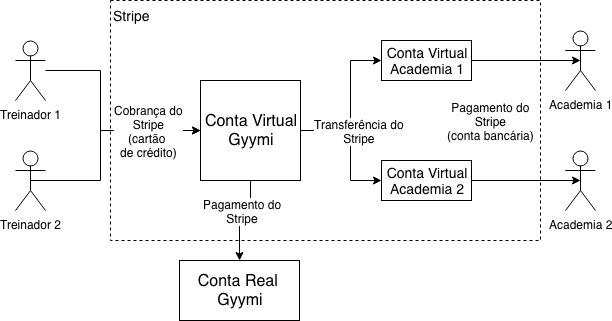
\includegraphics[width=0.8\textwidth]{pfc/figuras/payment-system-stripe.png}
    \caption{Funcionamento do sistema de pagamentos}
    \label{fig:payment-system}
\end{figure}

\begin{figure}[H]
    \centering
    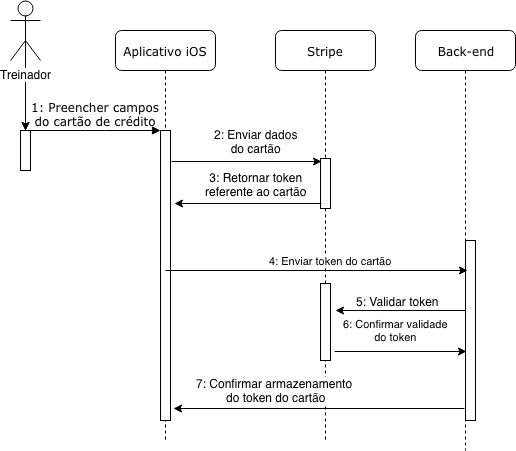
\includegraphics[width=0.8\textwidth]{pfc/figuras/seq-diagram-token.png}
    \caption{Diagrama de sequência da dinâmica de \textit{tokenização} do cartão de crédito}
    \label{fig:seq-diagram-token}
\end{figure}

A implementação dos esquemas apresentados não foi concluída para a fase piloto do aplicativo. Para o piloto, foi utilizado um ambiente fictício que o Stripe fornece para testes. Transações fictícias foram criadas no Stripe ao final dos agendamentos de treinos, emitindo-se cobranças em cartões de crédito fictícios.

\subsubsection{Envio de SMS}
O sistema de envio de SMS foi utilizado para cumprir o requisito funcional de envio de SMS para verificação de número telefônico. A verificação é feita somente no cadsatro de novos treinadores (Figura \ref{fig:register-trainer-verification}). O serviço utilizado foi o Twilio \todo{citar twilio}.

A dinâmica de envio de SMS é ilustrada no diagrama de sequência da Figura \ref{fig:seq-diagram-sms}. O sistema opera da seguinte forma: o usuário preenche o cadastro através da interface gráfica do aplicativo iOS, em especial o campo de número do celular; os dados de cadastro são enviados e validados no back-end, que faz uma chamada de API para o Twilio com um pedido de envio de SMS para o número de celular cadastrado; o usuário, então, preenche o campo de código de verificação no aplicativo com o código recebido via SMS; o código de verificação é enviado ao back-end, que realiza a validação do mesmo com o Twilio; por fim, uma confirmação da validação do código de verificação é enviada ao aplicativo iOS, permitindo que o usuário prossiga com o cadastro.

\begin{figure}[H]
    \centering
    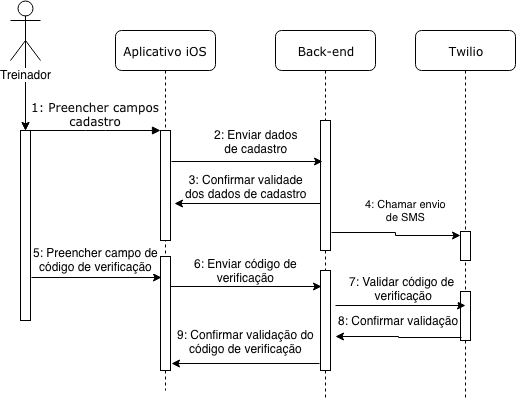
\includegraphics[width=0.8\textwidth]{pfc/figuras/seq-diagram-sms.png}
    \caption{Diagrama de sequência da dinâmica de envio de SMS para verificação de número telefônico}
    \label{fig:seq-diagram-sms}
\end{figure}

\subsection{Testes de RESTful API's}
Todas as integrações de sistemas apresentadas anteriormente foram realizadas utilizando RESTful API's. Com o intuito de agilizar e automatizar o processo de teste de chamadas de API, utilizou-se durante o projeto a ferramenta de software denominada Postman \todo{citar postman}. A ferramenta permite que conjuntos de chamadas de API's (coleções) sejam criadas, permitindo o teste das chamadas individualmente ou em conjunto (com o sequenciamento das chamadas).

A Figura \ref{fig:postman} ilustra a interface do Postman. Na esquerda, encontram-se as coleções, com as respectivas listas de chamadas de API. Na parte central superior, existem abas com as chamadas e seus parâmetros de configurações. Na parte central inferior, encontra-se um console onde a resposta da chamada é exibida.

\begin{figure}[H]
    \centering
    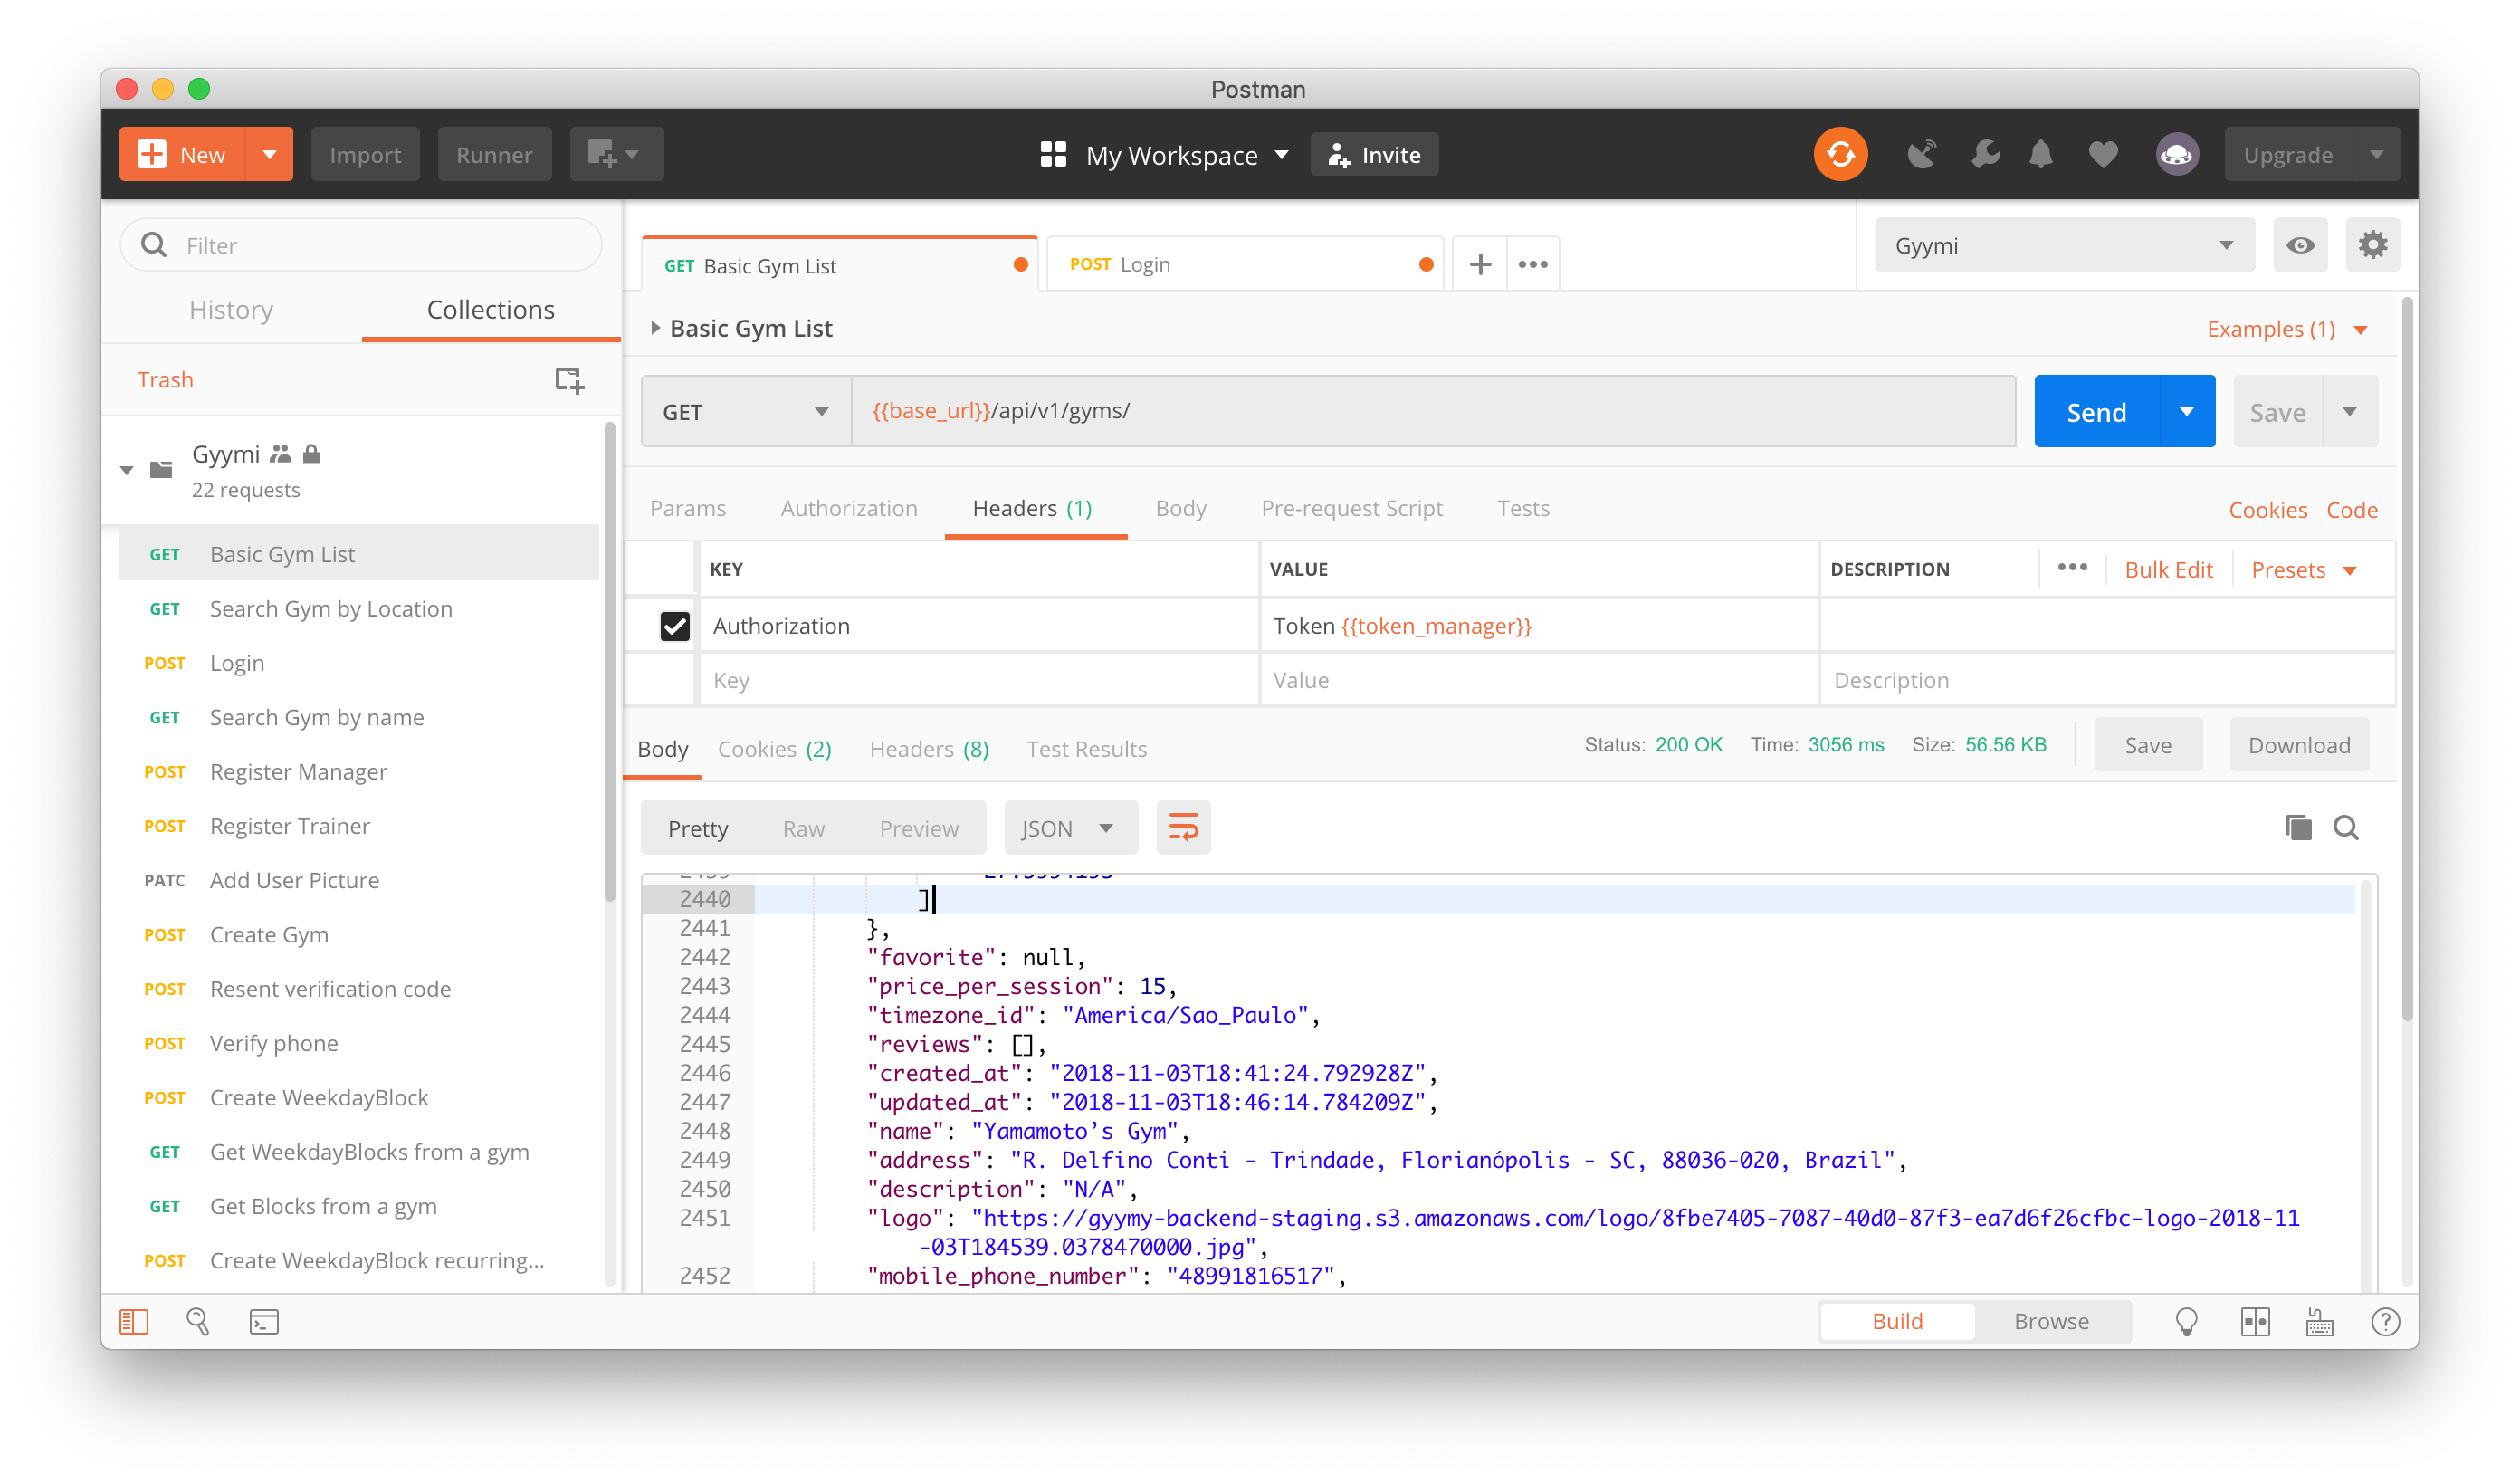
\includegraphics[eidth=0.8\textwidth]{pfc/figuras/postman.png}
    \caption{Postman - ferramente utilizada para testes de RESTful API's}
    \label{fig:postman}
\end{figure}

% *****************
% Interface Gráfica
% *****************
\section{Interface Gráfica}

criterio de testes e avaliacao

componentes reusaveis
botao
calendario
stepper
navbar

tratamento de erros
cadastro
regex
api

bibliotecas
image crop/resize
googlemapas


desafios/detalhes de implementação
espaço entre campos e botao
tamanhos de dispositivo
tabelas de horario
redirecionar insta/website
bolinha calendario

% ********************
% Testes Automatizados
% ********************
\section{Testes Automatizados de Interface Gráfica}

\subsection{Implementação dos Testes}

\subsubsection{EarlGrey}

\subsubsection{Appium}

\subsubsection{XCUITest}
